\chapter{Design and Implementation}\label{ch:design}

\section{Multiplexer Policy}

\subsection{Receive Policy}

\subsection{Round Robin Policy}

\subsection{Priority Based Policy}

\subsection{Bandwidth Limited Policy}

\subsection{Enforcing Policy Through System Design}


\section{Broadcast Protocols}
Some protocols broadcast traffic to all systems by addressing the
ethernet packet with a specific MAC address of ff:ff:ff:ff. However,
as the receive multiplexer is based on MAC addresses, it will not
know how to handle such packets. In particular, we need to support 
the address resolution protocol (ARP), as it maps an
IPv4 address to a MAC address and thus 
is required for any network communication via ethernet.\\
One possible solution is to copy these packets to all client applications.
This would require additional policy in the receive multiplxer that ensures
all client side receive free (RxF) queues have enough free buffers available
for the multiplexer to dequeue and then copy broadcast packets into.
However, there are many different broadcast protocols, for example the Dynamic
Host Configuration Protocol (DHCP), and the arrival of such packets
can be nondeterministic. This makes it difficult to determine how many might arrive
simultaneously and thus how many buffers should be available in all client side
RxF queues at all times. If there aren't any free buffers available for ARP, then
a client will not be able to receive any IPv4 traffic.\\
Instead, we implement a separate component to handle broadcast traffic. It interfaces
with the multiplexers the same as any other client, as shown in \autoref{f:mux}. 

\begin{figure}[h]
    \centering
    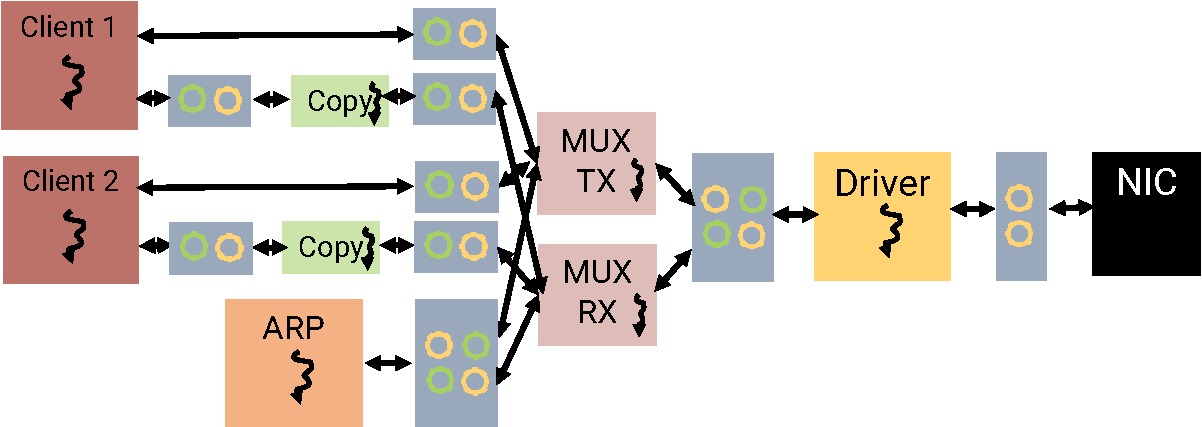
\includegraphics[width=\textwidth]{arp.pdf}
    \caption{Multiple client applications with an ARP component on the sDDF}
    \label{f:arp}
\end{figure}

\subsection{Separate ARP Component}
A separate ARP component only requries the minimal functionality to respond to 
the address resolution protocol on behalf of any client applications running on
the system. In keeping with the design goals, this component will be kept 
very simple in the aims of enabling formal verification. Therefore we consider
this component to be trusted to maintain the integrity of its shared queues with
the multiplexer components as well as interfacing with clients and responding
correctly to ARP on behalf of the clients. \\
While supporting other broadcast protocols, such as DHCP, is out of scope of this thesis, 
the simplicity of the ARP component design enables its functionality to be extended easily
to support other broadcast protocols in the future.

\subsection{Client Interface}
As ARP is based on both MAC addresses and IPv4 addresses, the new component
requires an interface with client applications. This interface will allow clients
to register a new IPv4 address, change an IPv4 address, or remove one. As adding,
changing and removing an IPv4 address is typically very infrequent for networking systems
and requires minimal data exchange, we define this interface using a protected procedure
call (PPC) from the client to the ARP component. 

\begin{minipage}{\textwidth}
    \centering
    \begin{lstlisting}[tabsize=2, language=C, caption={Client Interface to ARP Component},frame=tb, 
                        label={l:queues2}, captionpos=b]
        void register_ip4(new_ip4_addr, mac_addr[6])
        {
            /* split the MAC address across two registers so it fits */
            sel4cp_mr_set(0, mac_addr[0:4]);
            sel4cp_mr_set(1, mac_addr[4:6]);
            sel4cp_mr_set(2, new_ip4_addr);
            sel4cp_ppcall(ARP, sel4cp_msginfo_new(REGISTER_IP, 3));
        }

        void change_ip4(old_ip4_addr, new_ip4_addr, mac_addr[6])
        {
            sel4cp_mr_set(0, mac_addr[0:4]);
            sel4cp_mr_set(1, mac_addr[4:6]);
            sel4cp_mr_set(2, old_ip4_addr);
            sel4cp_mr_set(3, new_ip4_addr);
            sel4cp_ppcall(ARP, sel4cp_msginfo_new(CHANGE_IP, 4));
        }

        void remove_ip4(old_ip4_addr, mac_addr[6])
        {
            sel4cp_mr_set(0, mac_addr[0:4]);
            sel4cp_mr_set(1, mac_addr[4:6]);
            sel4cp_mr_set(2, old_ip4_addr);
            sel4cp_ppcall(ARP, sel4cp_msginfo_new(REMOVE_IP, 3));
        }
    \end{lstlisting}
\end{minipage}

Currently, the ARP component can only store a single IPv4 address per client, which
is enough for our testing purposes, however this limit can be extended easily in the code
base should the need arise.


\section{Client Applications}

\subsection{Asymmetric Traffic}
\subsection{Client Initiated Transmit}
